\documentclass[11pt]{article}
\usepackage[utf8]{inputenc}
\usepackage{textcomp}
\usepackage[letterpaper,margin=1in]{geometry}

\newcommand{\textunderscript}[1]{$_{\text{#1}}$}
\usepackage{relsize}
\usepackage{amsmath}

\usepackage{graphicx}

\usepackage{hyperref}
\usepackage{pdfpages}

\usepackage{fancyhdr}
\pagestyle{fancy}
\fancyhf{}
\rhead{\thepage}
\lhead{Structures and Multidisciplinary Optimization Group}

\title{GitHub Guide for the Structures and Multidisciplinary Optimization Group}
\author{Brian Burke and Yicong Fu}
\date{May 2022}

\begin{document}

\maketitle
\thispagestyle{fancy}

\section{Overview}
GitHub is an online service that hosts tools for software development and version control using Git. Git is an open-source software that is commonly used for coordination among programmers during software development. Git offers distributed version control and source code management to enable programmers to work on the same project across various branches of code and on various machines. Git can be installed from \url{https://git-scm.com/downloads}. Git is commonly used as a command line tool; a cheat sheet from \url{https://education.github.com/git-cheat-sheet-education.pdf} has been included as an appendix to this document. Note that GitHub graphical user interfaces are also available as downloads for Windows and Mac--see the same cheat sheet for respective links.

\subsection{Git}
There are two main ingredients of git: the remote repository and the local copy.
The remote repository is the server where a code is stored. It is where you can get the code from by \emph{pulling} or upload your changes by \emph{pushing}.
The local copy is the local repository stored on your workstation. You can make changes to this local copy using a code editor or terminal interface. Changes are then added to the history of your local copy through \emph{commits}, which help to organize changes to the code in a log format. The remote repository is only updated when you \emph{push} to it. 
Once you feel comfortable with the changes you've made locally, you can \emph{push} your \emph{commits} to the remote repository to share your progress with your collaborators. Other people can then \emph{pull} your changes to their own local copies to keep their code updated.

Basic git only has command line interface (CLI).
If you need a GUI you could download GitHub Desktop.
In terms of how git works and how to use git CLI, there are many good references out there. The following ones are a few beginner-level tutorials:

\begin{itemize}
    \item \href{https://missing.csail.mit.edu/2020/version-control/}{https://missing.csail.mit.edu/2020/version-control/}
    \item \href{https://learngitbranching.js.org/}{https://learngitbranching.js.org/}
\end{itemize}

\subsection{GitHub}
Git repositories can be hosted either on local machine, on some server in the local network, or on the internet.
GitHub is one of the biggest service providers of internet hosting for git repositories.
There are two main versions of GitHub: public (github.com) and enterprise (e.g., github.gatech.edu).
These are separate from each other. However, the SMDO group will generally be using the public GitHub only.
The following sections will cover the new workflow.

\section{Workflow}
\subsection{Prerequisites}
First, make sure you have an account for public GitHub and git on your local machine, which is usually preinstalled on Unix-like systems (but not for Windows).

Next, register this account on your local machine to let git know who you are.
This can be done by running the following commands in terminal from anywhere:

\texttt{git config --global user.name your-account-name}

\texttt{git config --global user.email your-account-email}

The commands above will write account information to your global git configuration file, which is in \texttt{\$HOME/.gitconfig}
for Linux and MacOS.
Notice that if you also have other projects under a different github account (e.g., another github.com account
or an enterprise account), you will need to set it up separately by running the following
commands in the project folder in terminal:

\texttt{git config user.name your-account-name}

\texttt{git config user.email your-account-email}

\noindent These commands essentially write to a repository-specific configuration file located in: \newline \indent \texttt{project-folder/.git/config}.

\noindent In order to prevent some issues when pulling, you will also need to do run:

\texttt{git config --global pull.ff only}

\subsection{Fork and Pull Method}
The SMDO group uses the \emph{Fork and Pull} model for collaborative development. Under this method, anyone can fork an existing repository to their own account where they are free to make changes to their personal fork. The repositories on the \url{https://github.com/smdogroup} organization page serve as the base/parent repositories for all major software projects under development in the SMDO group. Individuals may make changes and commits as necessary to get new code working. Once your personal fork is working and passes any applicable tests, you can open a \emph{pull} request from your fork to the parent repository. The pull requests allows users to discuss and review changes to the code before merging into the base repository. After a successful review by one of the project maintainers, the pull request will be merged into the main branch.
\begin{enumerate}
    \item You should work from your own fork of the main \verb|github.com/smdogroup| repositories. This is easily done using the web interface and clicking the ``fork" button on the respective repository. This will create a separate repository under your own account.
    \item Clone your fork to your local machine. Check for any references to other repositories with \verb|git remote -v|; delete these extraneous references. Set the origin as your personal GitHub fork. Notice that ``fork'' is a GitHub specific feature which git doesn't have.
    So once you clone the repo, anything you do with \texttt{git} command will only
    affect your ``forked'' repo, but not the ``upstream'' repo under smdogroup's account.
    This can be verified by running:

    \texttt{git remote --verbose}

    And you will only see the urls of your own remote repo (but not the repo under smdogroup).
    \item Create a new branch under your repo for the feature you'll be working on.
    The name of the branch should be precise and self-explanatory.
    This can be done either on the GitHub webpage or locally by running the
    following command \textbf{on the branch you're branching from (for example master)}:

    \texttt{git checkout -b name-of-your-branch}

    which will create a new branch and switch to it.
    Then you can do:

    \texttt{git branch}

    to verify that you're at the correct branch.

    Note:
    Branching is implemented in a very cheap way for git, and it makes the code base organized
    if many different features are developed at the same time.
    so it's a good practice to always make a branch for certain task. It is discouraged to commit directly to master (or main, which is GitHub's new nomenclature) branch, even for your own forked repository.
    
    \item Now you are ready to work on the code. You can commit as many times as you want to your branch. \textbf{Before making changes}, be sure to pull from the main github repo to your fork. Then pull to your local copy using \verb|git pull origin| or \verb|git fetch origin|. This is done in case there are new changes in the remote repository or the main repository that you don't have locally.
    
    It's recommended to frequently push local changes to GitHub, so that you will always have backups online.
    You can only push \emph{commits} (but not uncommitted changes) so make sure to commit before push.
    
    \item While we are working on the local fork, the upstream repo might change. Therefore, you need to periodically update your local fork.
    This needs to be done on the GitHub webpage, by simply clicking the ``Fetch upstream'' button.
    If there are indeed updates from upstream, you might also need to update your branch.
    This is because your branch was originated from some other branch (likely the master),
    which might be updated by such action.
    You can update your branch by:

    \texttt{git checkout name-of-your-branch \&\& git merge branch-to-update-from}
    
    \item
    Once you feel comfortable with your changes, it's time for the main repo to incorporate your
    contributions!
    This will be done via ``pull request'', which is another GitHub specific feature that git doesn't
    have. So you will need to go to the GitHub webpage and open a pull request ticket. Although the term might be confusing, it can be thought of as ``to request a pull to main from you".
    The pull request should be from your repo to smdogroup/repo, and usually it'll be to the master branch.
    The pull request then will be reviewed, tested, and finally approved and merged (hopefully).
    
    To make it easier for the project maintainers (those who will be reviewing your pull requests), it is important to \textbf{include thorough documentation in your pull requests}. Inside a pull request, it is also possible to make new commits, write comments, and add replies. In this way, a pull request can form a place to discuss proposed changes before they are implemented in the main repository.

    \item
    Once the pull request is approved, you should delete the local branch you've been working on.
    Never keep working on the merged branch and ``pull request'' again in the future,
    because it and will cause redundant commit history to the master branch.

    \item
    Lastly, you will do a final ``Fetch upstream'', then your work will be reflected in the master
    branch of your own forked repo.
    And do another \texttt{git pull} locally to download the updates.

\end{enumerate}

\clearpage
 \ 
\vfill
\begin{figure}[h]
    \centering
    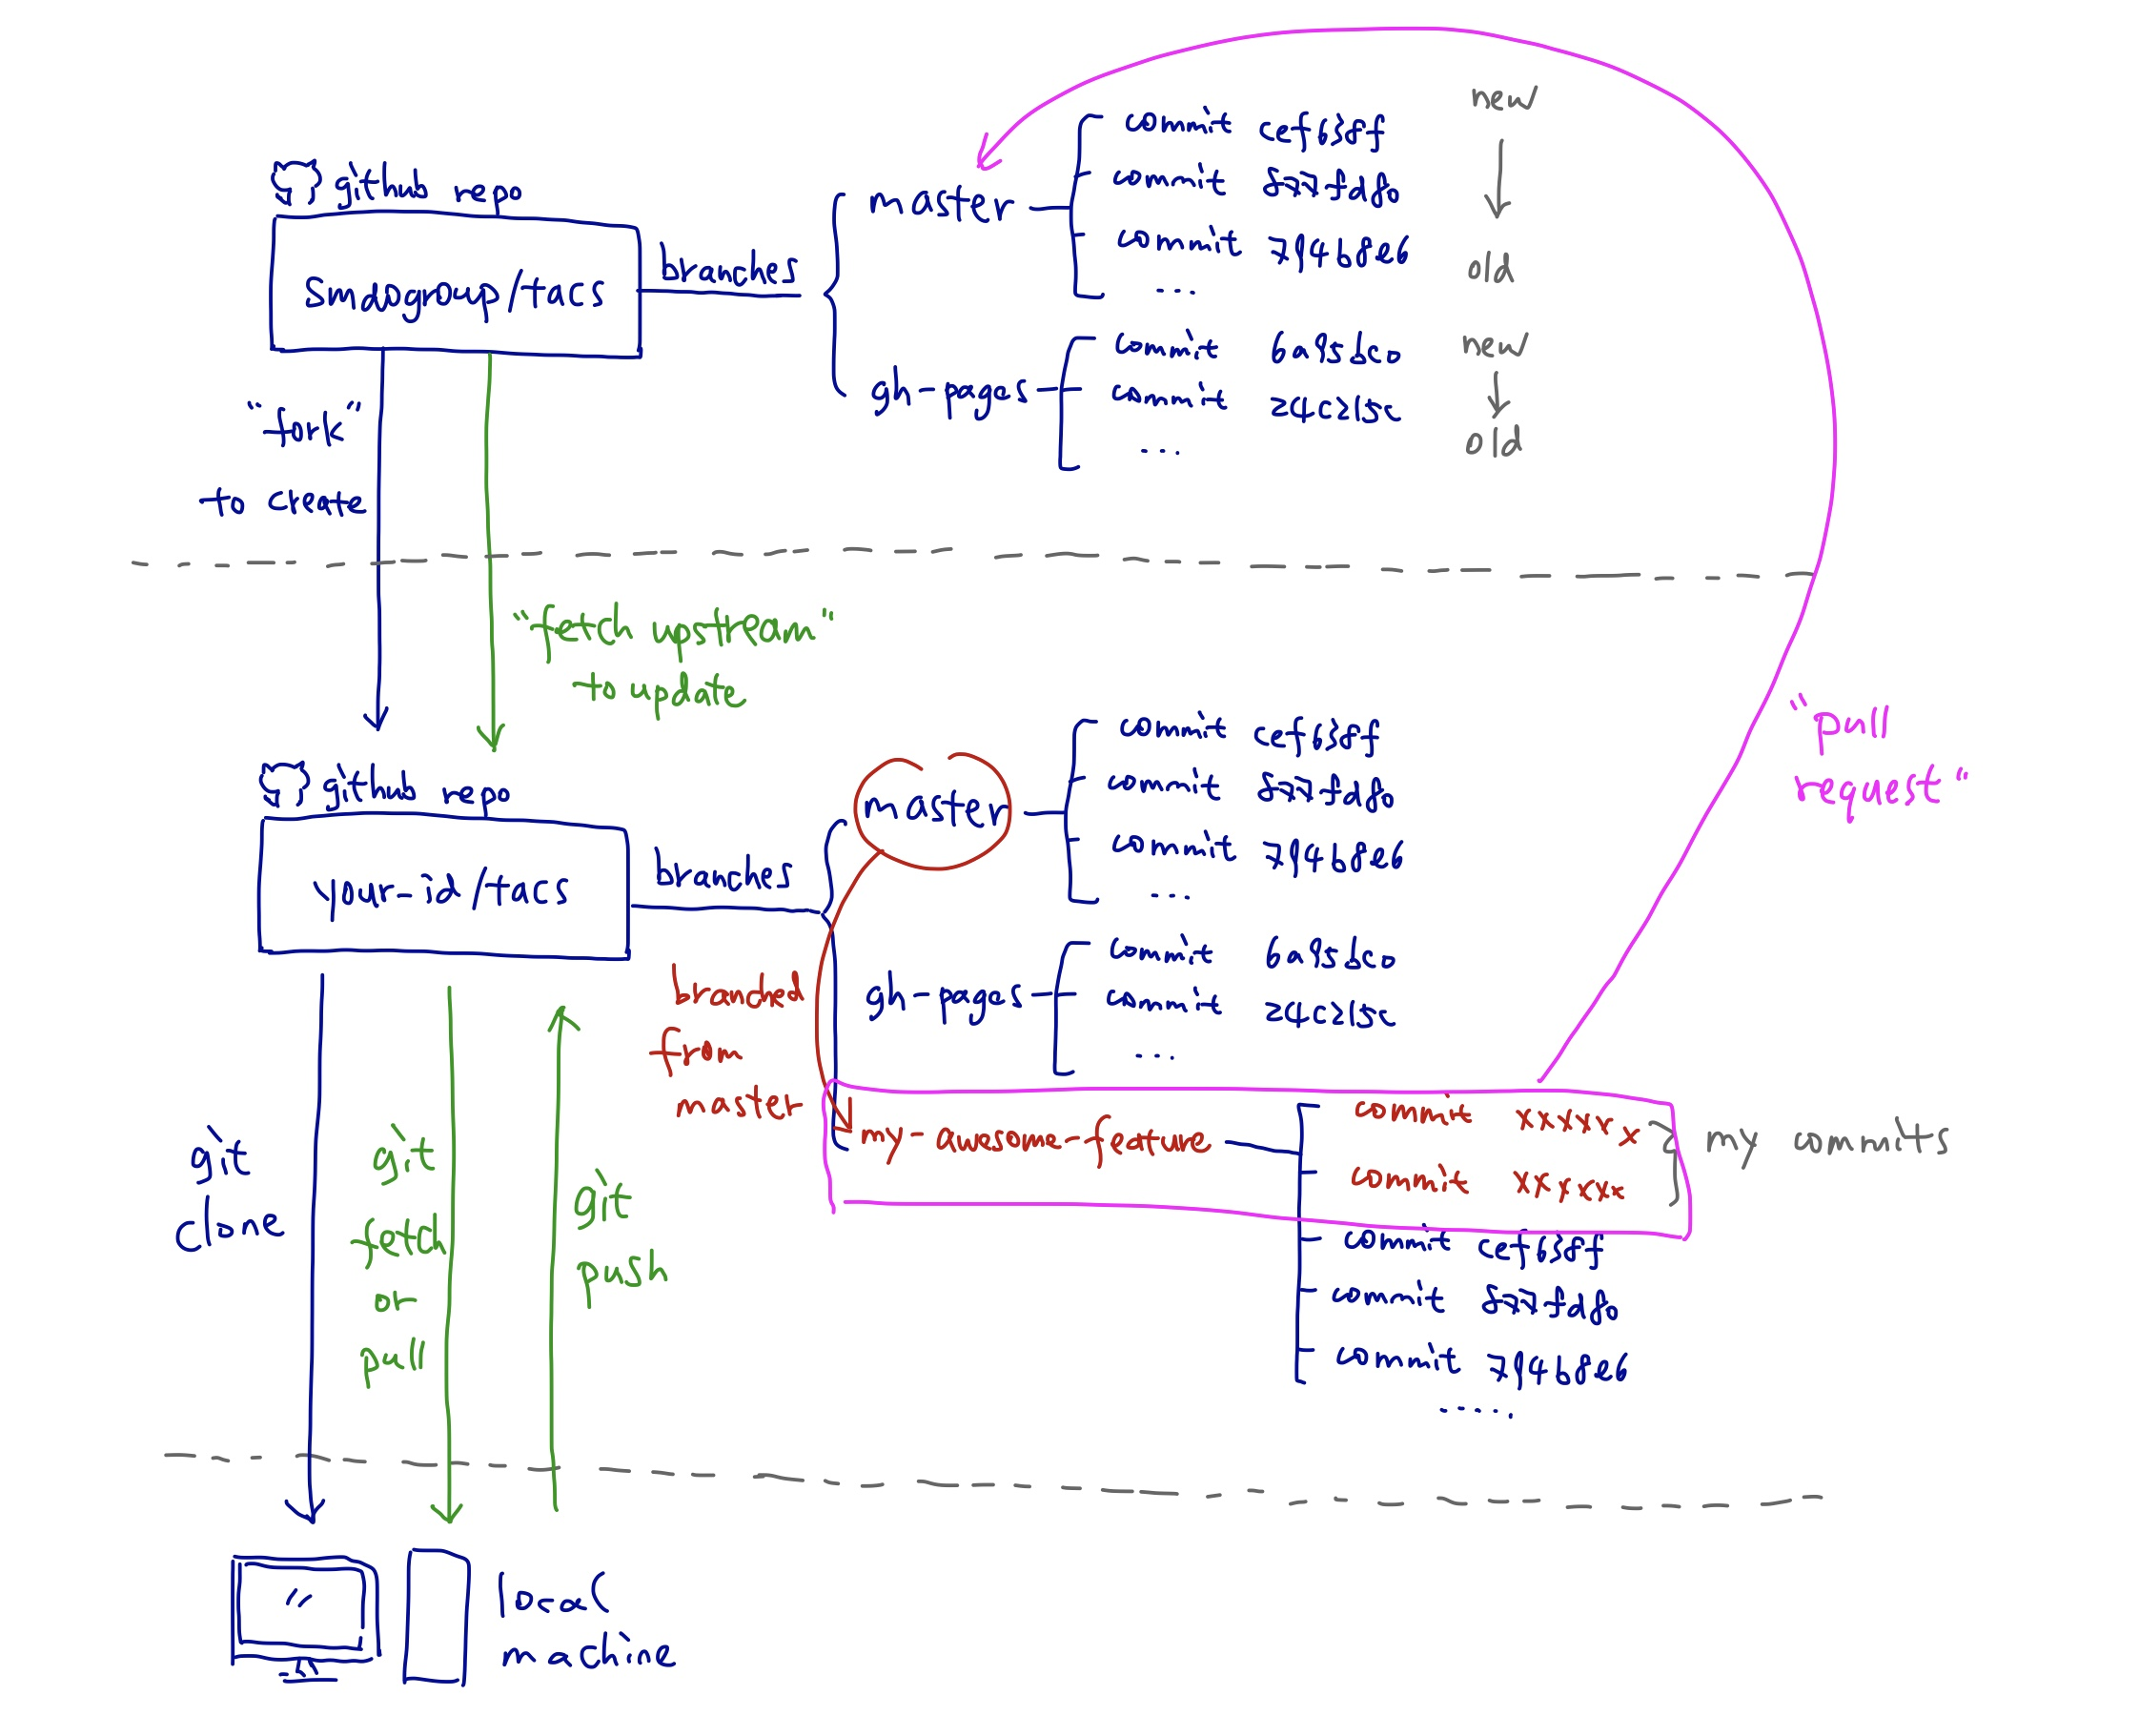
\includegraphics[width=\textwidth]{pics/cartoon.jpg}
    \label{fig:cartoon}
    \caption{Git/github workflow diagram}
\end{figure}
\vfill

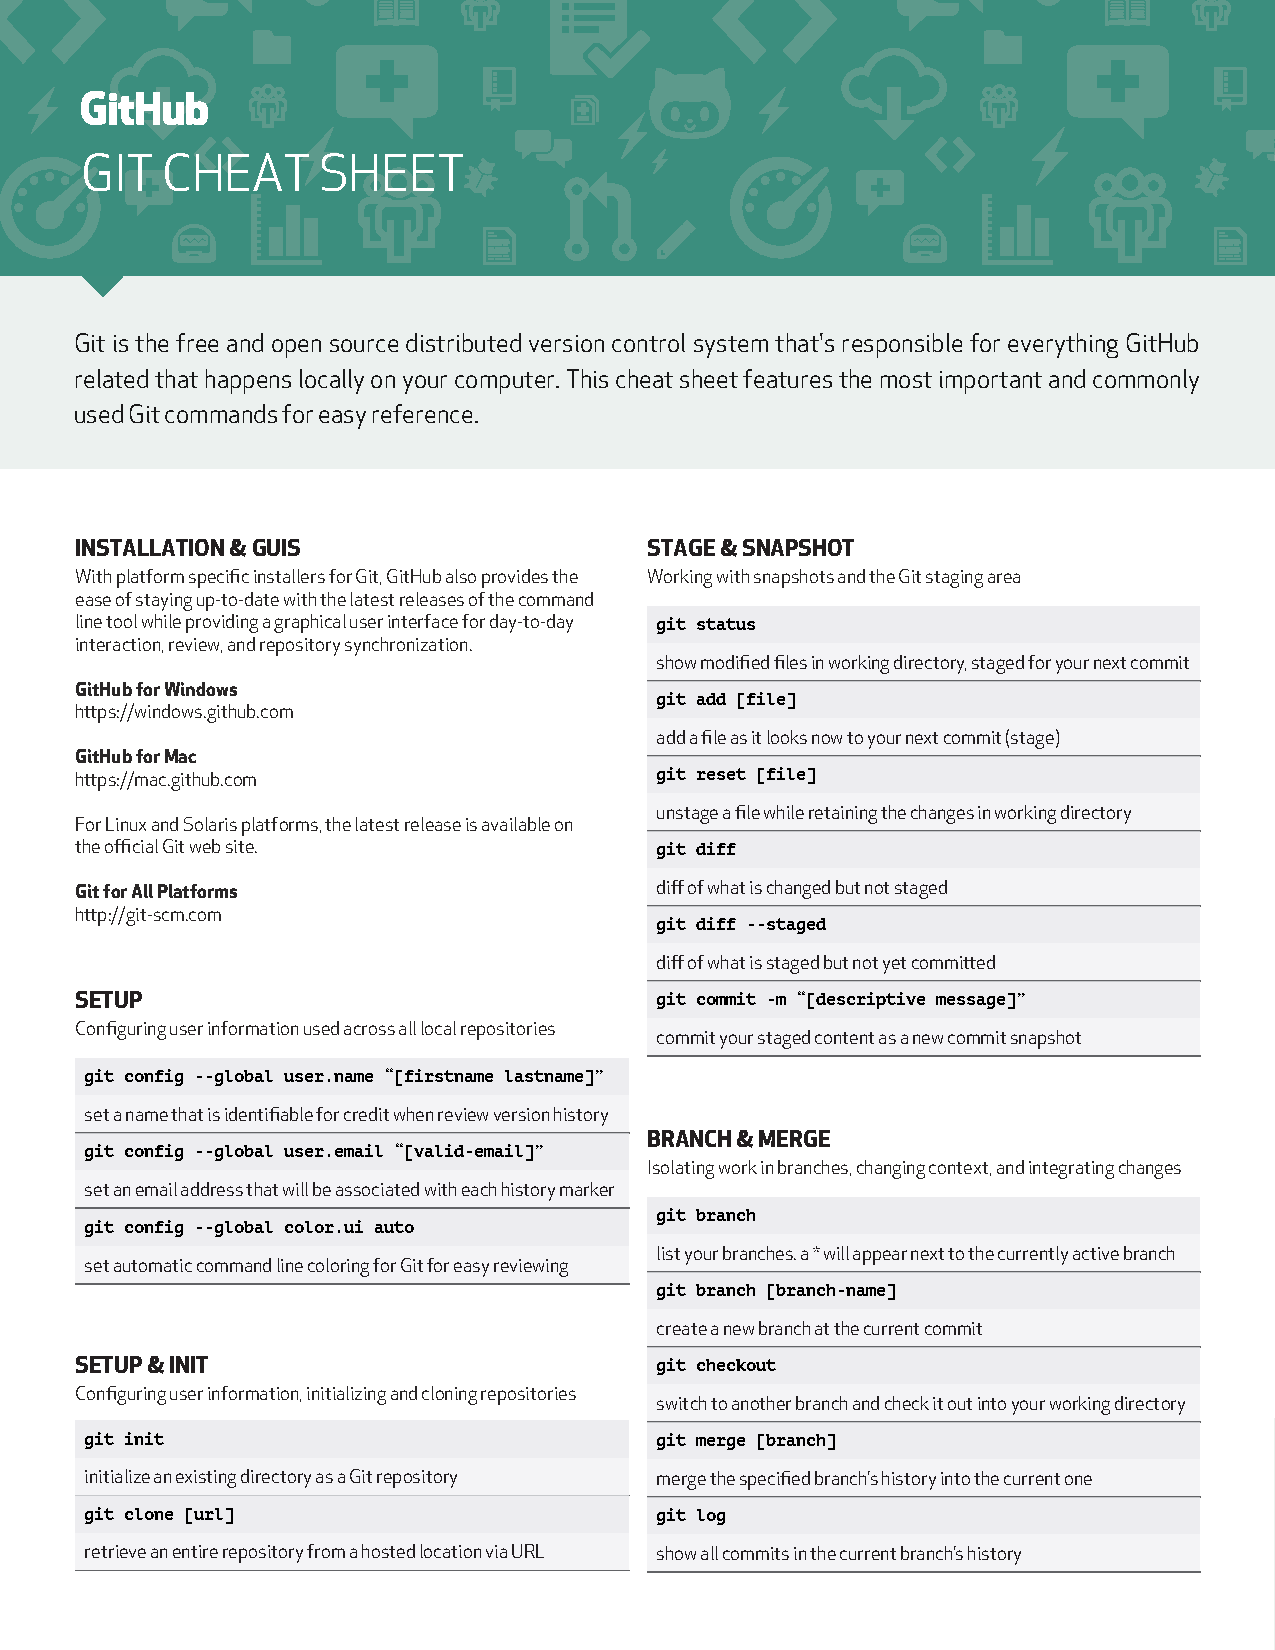
\includepdf[pages=-]{git-cheat-sheet-education.pdf}
\end{document}
